\documentclass[tikz, margin=5mm]{standalone}

%%% This file contains definitions of shapes and nodes used
%%% for a recipe workflow
%%% Author       : Oliver Czoske
%%% Created      : 2021-03-03
%%% Last Changed : 2021-03-03
%%% Changes:
%%%

\usetikzlibrary{
  shapes.misc,
  positioning,
  calc,
  arrows.meta}

%% All connecting lines have an arrow
\tikzset{
  connection_arrow/.style={->, >=Latex[open], thick}
}

%% Start and stop buttons (black disks, stop with ring)
%% These are pics, use as
%%         \pic (name) [above of=..] {picname};
\tikzset{
  start/.pic = {
    \node (-m) at (0, 0){};
    \filldraw [fill=black] (0, 0) circle (0.2);
  }
}

\tikzset{
  stop/.pic = {
    \node (-m) at (0, 0){};
    \node (-t) at (0, -0.3){};
    \filldraw [fill=black] (0, 0) circle(0.2);
    \draw[black] (0, 0) circle (0.3);
  }
}


%%%% Various boxes and their colours
%%%% These are nodes, use as
%%%% \node (name) [type, location]  {text};

\definecolor{stepcolor}{RGB}{210,169,188}
\definecolor{rawcolor}{RGB}{205,205,205}
\definecolor{externalcolor}{RGB}{183,255,255}
\definecolor{calibcolor}{RGB}{255,250,216}
\definecolor{calproductcolor}{RGB}{185,184,237}
\definecolor{qcproductcolor}{RGB}{255,201,165}
\definecolor{sciproductcolor}{RGB}{197,219,183}
\definecolor{framecolor}{RGB}{127,13,65}

\tikzset{
  %% template : the template(s) that trigger(s) the recipe
  template/.style={
    rectangle,
    draw=black,
    minimum width=4.0cm,
    minimum height=0.5cm,
    align=center
  },
  %% input : the input files
  input/.style={
    rectangle,
    fill=rawcolor,
    minimum width=4.0cm,
    minimum height=0.75cm,
%     text width=3cm,
    align=center
  },
  %% calib : calibration input
  calib/.style={
    rectangle,
    fill=calibcolor,
    minimum width=4.0cm,
    minimum height=0.75cm,
%     text width=3cm,
    align=center
  },
  %% external : external input
  external/.style={
    rectangle,
    fill=externalcolor,
    minimum width=4.0cm,
    minimum height=0.75cm,
%     text width=3.5cm,
    align=center
  },
  %% params : parameters
  params/.style={
    rectangle,
    draw=red,
    thick,
    minimum width=4.0cm,
    minimum height=0.75cm,
%     text width=3cm,
    align=center
  },
  %% redstep : a reduction step
  %%      ("step" is predefined and can't be used)
  redstep/.style={
    rectangle,
    rounded corners=0.2cm,
    fill=stepcolor,   %%% define colour!
    minimum width=4.0cm,
    minimum height=1cm,
%     text width=3cm,
    align=center
  },
  %% connection : connection to input or output
  connection/.style={
    circle,
    fill=black,
    minimum size=0.15cm,
    inner sep=0pt
  },
  %% sciproduct : a science product
  sciproduct/.style={
    rectangle,
    fill=sciproductcolor,
    minimum width=4.0cm,
    minimum height=0.75cm,
%     text width=3.5cm,
    align=center
  },
  %% calproduct : a calibration product
  calproduct/.style={
    rectangle,
    fill=calproductcolor,
    minimum width=4.0cm,
    minimum height=0.75cm,
%     text width=3.5cm,
    align=center
  },
  %% frame : frame around the recipe
  %% This is a path, use as
  %%    \draw [frame] (upper left) rectangle (lower right);
  frame/.style={framecolor, very thick, dashed}
}


\begin{document}

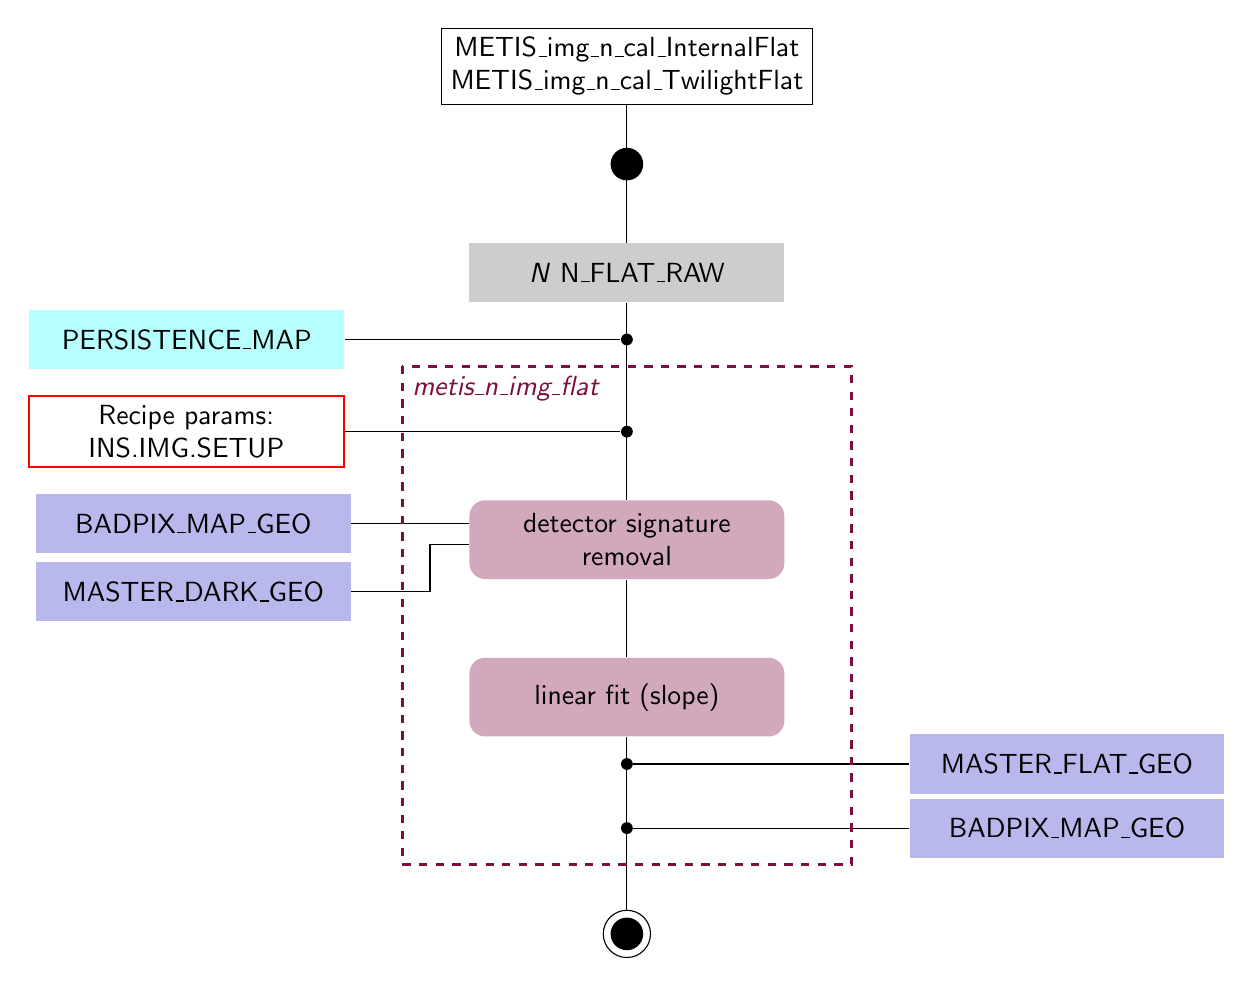
\begin{tikzpicture}
  [x=1cm,
  y=-1cm,
  align=center,
  node distance=2cm and 3.5cm]
  \sffamily

  %% Grid for orientation. Comment out for final figure!
  % \draw[help lines, green](-5, 0) grid (8, 11);

  %%% Put workflow commands here:
  %% Main reduction workflow

  \node (template) [template] {%
    METIS\_img\_n\_cal\_InternalFlat\\
    METIS\_img\_n\_cal\_TwilightFlat};

  \pic (start)[below=0.75cm of template]{start};

  \node (input) [below=0.75cm of start-m, input] {%
    \textsl{N} N\_FLAT\_RAW};

  \node (step1) [below=2.5cm of input, redstep]{%
    detector signature\\ removal};

  \node (step2) [below of=step1, redstep]{%
    linear fit (slope)};

  \pic (stop) [below=2.5cm of step2] {stop};

  %% Connections
  \draw (template) -- (input);
  \draw (input) -- (step1);
  \draw (step1) -- (step2);
  \draw (step2) -- (stop-t);

  %% Output
  \node (connectpers) [connection] at
  ($(input)!0.25!(step1)$){};
  \node (persistence) [left=of connectpers, external]{%
    PERSISTENCE\_MAP};
  \draw (persistence) -- (connectpers);

  \node (connectparams) [connection] at
  ($(input)!0.7!(step1.north)$){};
  \node (params) [left=of connectparams, params]{%
    Recipe params:\\
    INS.IMG.SETUP};
  \draw (params) -- (connectparams);

  \node (bpmin) [left=of step1.center, yshift=0.2cm, calproduct]{%
    BADPIX\_MAP\_GEO};
  \draw (bpmin.east) -- ++(1.5,0);

  \node (darkin) [below=0.1cm of bpmin, calproduct]{%
    MASTER\_DARK\_GEO};
  \draw (darkin.east) -- ++(1.0,0) -- ++(0,-0.6) -- ++(0.5,0);

  \node (connectflat) [connection] at
  ($(step2)!0.3!(stop-t)$){};
  \node (flatout) [right=of connectflat,calproduct]{%
    MASTER\_FLAT\_GEO};
  \draw (connectflat) -- (flatout);

  \node (connectbpm) [below=0.65cm of connectflat, connection]{};
  \node (bpmout) [right=of connectbpm, calproduct]{%
    BADPIX\_MAP\_GEO};
  \draw (connectbpm) -- (bpmout);

  %% Frame around recipe
  \draw [frame] ($(input)!0.35!(step1) -(2.85,0)$) rectangle
  ($(step2)!0.75!(stop-t) + (2.85,0)$);
  \node [framecolor, anchor=north west] at
  ($(input)!0.35!(step1) - (2.85,0)$){%
    \textsl{metis\_n\_img\_flat}};

\end{tikzpicture}

\end{document}
